\documentclass{article}
\usepackage{url}
\usepackage{fancyhdr}
\usepackage{amsmath, amsfonts, amsthm, amssymb}  
\usepackage{secdot}
\usepackage{epsfig}
\usepackage{lastpage}
\usepackage{hyperref}
\usepackage{graphicx}
\usepackage{color}
\usepackage{epstopdf}
\usepackage{fancyvrb}

\usepackage{geometry}
\geometry{letterpaper, left=1in, right=1in, top=1in, bottom=1in}

\pagestyle{fancy}
\fancyhf{}
\renewcommand{\headrulewidth}{0pt}
\rfoot{\thepage/\pageref{LastPage}}
\lhead{OSU ECEN 4233 - High-Speed Computer Arithmetic - Spring 2021}
\lfoot{\LaTeX}

\begin{document}

\title{Dadda Multiplier Example}
\author{James E. Stine \\
Electrical and Computer Engineering Department\\
Oklahoma State University \\
Stillwater, OK 74078, USA}
\date{}

\maketitle
%\thispagestyle{plain}\pagestyle{plain}

\section{Dadda Multiplier}
This document is meant to show the in-class example of a $6$-bit by $6$-bit
Dadda Multiplier.  
Here is
a table documenting the area where the final iteration has an $10$-bit CPA:
  \begin{table} [h]
    \centering
    \begin{tabular}{|c|c|c|c|c|c|c|c|c|c|} \hline
    Iteration & Number of $(3,2)$ Counters & Number of $(2,2)$ Counters \\
    \hline \hline
      1 & 3 & 3  \\ \hline
      2 & 5 & 1  \\ \hline
      3 & 7 & 1  \\ \hline \hline
  Total & 15 & 5 \\ \hline
    \end{tabular}
  \end{table}

The methodology
for creating Dadda trees, or so they are called, can
be organized into the following steps listed below.  
\begin{enumerate}
\item Reorganize matrix into inverted triangle (optional)
\item Figure out where the partial product matrix height falls within the
  Dadda sequence.  Remember the series is found by multiplying a height by
  $3/2$ and flooring it,
  \begin{eqnarray*}
  height_0 & = & 2 \\
  height_{i+1} & = & \lfloor height_i \times 3/2 \rfloor 
  \end{eqnarray*}
\item Draw a dashed line between at the Dadda sequence you need to get to.
\item Starting at far right column, use $(2,2)$ and $(3,2)$ counters to
  reduce the stage until the Dadda sequence is met.
\item Repeat step $(3)$ until the final height is $2$.
\end{enumerate}

  \begin{figure}
    \begin{center}
      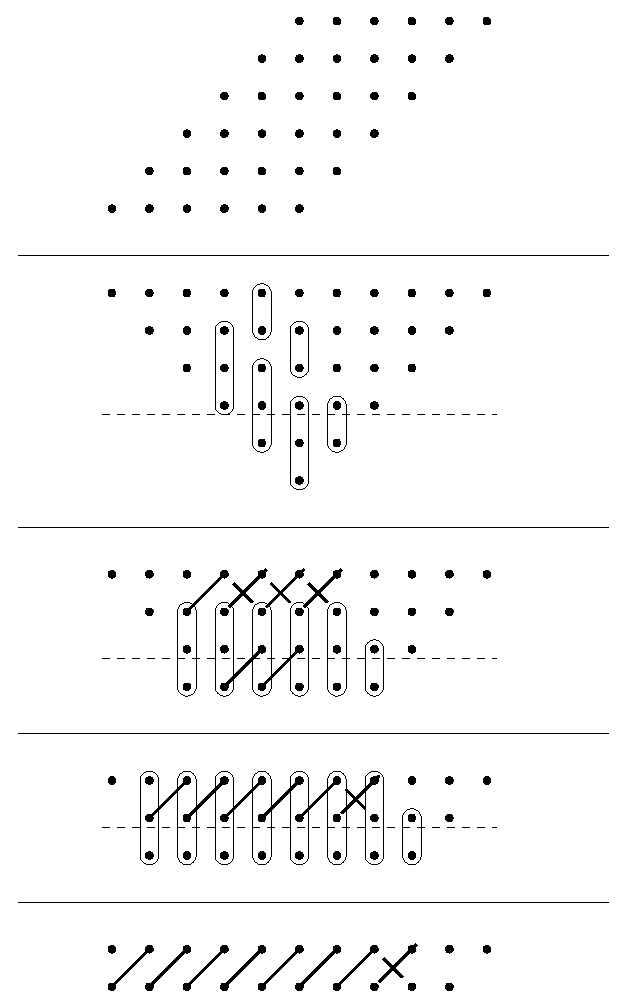
\includegraphics[scale=1.0]{dadda6.eps}
    \end{center}
    \label{wallace6.fig}
    \caption{In-class Example of $6 \times 6$ Dadda Multiplier.}
  \end{figure}

\end{document}
